\documentclass{beamer}
\usepackage[utf8]{inputenc} % make weird characters work
\usepackage[english,serbian]{babel}
%\usetheme{Pittsburgh}
%\usecolortheme{beetle}
\setbeamertemplate{navigation symbols}{}

\usepackage{listings}
\usepackage{textcomp}
\usepackage{xcolor}

% \setmonofont{Consolas}
\definecolor{bluekeywords}{rgb}{0,0,1}
\definecolor{greencomments}{rgb}{0,0.5,0}
\definecolor{redstrings}{rgb}{0.64,0.08,0.08}
\definecolor{xmlcomments}{rgb}{0.5,0.5,0.5}
\definecolor{types}{rgb}{0.17,0.57,0.68}

\usepackage{amsmath}

\usepackage[figure]{algorithm}
\floatname{algorithm}{Pseudokod}
\usepackage{algorithmicx}
\usepackage{algorithm} 
\usepackage[noend]{algpseudocode}

\usepackage{listings}
\lstset{
    language=csh,
    captionpos=b,
    % aboveskip=5pt,
    % belowskip=5pt,
    numbers=left, 
    numberstyle=\tiny,
    frame=single,
    framesep=10pt,
    showspaces=false,
    showtabs=false,
    breaklines=true,
    showstringspaces=false,
    breakatwhitespace=true,
    escapeinside={(*@}{@*)},
    commentstyle=\color{greencomments},
    morekeywords={partial, var, value, get, set},
    keywordstyle=\color{bluekeywords},
    stringstyle=\color{redstrings},
    basicstyle=\ttfamily\footnotesize,
    tabsize=4,
    framexleftmargin=1.5em,
    xleftmargin=2em,
    % escapechar=\&,
    classoffset=1, 
    morekeywords={ until, final, abstract, event, new, struct,
    as, explicit, null, switch,
    base, extern, object, this,
    bool, false, operator, throw,
    break, finally, out, true,
    byte, fixed, override, try,
    case, float, params, typeof,
    catch, for, private, uint,
    char, foreach, protected, ulong,
    checked, goto, public, unchecked,
    class, if, readonly, unsafe,
    const, implicit, ref, ushort,
    continue, in, return, using,
    decimal, int, sbyte, virtual,
    default, interface, sealed, volatile,
    delegate, internal, short, void,
    do, is, sizeof, while,
    double, lock, stackalloc,
    else, long, static,
    enum, namespace, string, begin,
    declare, function, algorithm, integer,
    procedure,
    >,<,.,;,,,-,!,=,~},
    classoffset=0,
}

\usepackage[font=scriptsize,labelfont=bf]{caption}

\title{Jezi\v{c}ki invarijantna provera semanti\v{c}ke ekvivalentnosti strukturno sli\v{c}nih segmenata imperativnog koda}
\author{\href{mailto:ivan_ristovic@math.rs}{Ivan Ristovi\'c}}
\date{}


\begin{document}


\begin{frame}
    \titlepage
\end{frame}

\begin{frame}{Teme}
    \begin{itemize}
        \item Motivacija i uvod
        \item AST
        \item Dobijanje AST - ANTLR
        \item Op\v{s}ti AST
        \item Poređenje op\v{s}tih AST
        \item LICC --- Language Invariant Code Comparer
    \end{itemize}
\end{frame}

\begin{frame}[fragile]
\frametitle{Motivacija i uvod}
\begin{lstlisting}
void array_sum(int[] arr, int n) {
    int sum = 0, i = 0;
    while (i < n) {
        int v = arr[i]
        sum += v;
        i++;
    }
    return sum;
}
\end{lstlisting}
\begin{lstlisting}
function array_sum(arr, n)
    local sum = 0
    for i,v in ipairs(arr) do
        sum = sum + v
    end
    return sum
end
\end{lstlisting}
\end{frame}

\begin{frame}{Uvod i motivacija}
    \begin{itemize}
        \item Pristup?
        \begin{itemize}
            \item "Niski" pristup
            \item "Visoki" pristup 
        \end{itemize}
        \item Razlika je u reprezentaciji na koju se dovode segmenti koda pre procesa poređenja
        \item Ako je reprezentacija uvek ista, analiza je lakša
    \end{itemize}
\end{frame}

\begin{frame}{Uvod i motivacija}
    \begin{itemize}
        \item Niski pristup
        \begin{figure}[h!]
            \centering
            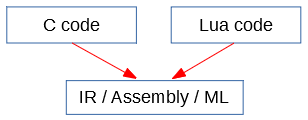
\includegraphics[scale=0.8]{images/approach_1.PNG}
        \end{figure}
        \item Prednosti: ista reprezentacija (?)
        \item Mane: vezanost sa specifi\v{c}nom arhitekturom procesora, potrebno prevoditi kod, JVM/CLR, razliciti programski jezici?
    \end{itemize}
\end{frame}

\begin{frame}{Uvod i motivacija}
    \begin{itemize}
        \item Visoki pristup (varijanta 1)
        \begin{figure}[h!]
            \centering
            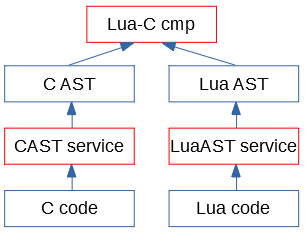
\includegraphics[scale=0.8]{images/approach_2.PNG}
        \end{figure}
        \item Prednosti: ista reprezentacija (?), nije potrebno prevoditi kod, kompatibilno sa bilo kojim programskim jezikom, mogu\'c{}e koristiti algoritme za poređenje stabala
        \item Mane: zavisnost od eksternih servisa, skaliranje
    \end{itemize}
\end{frame}

\begin{frame}{Uvod i motivacija}
    \begin{itemize}
        \item Visoki pristup (varijanta 2)
        \begin{figure}[h!]
            \centering
            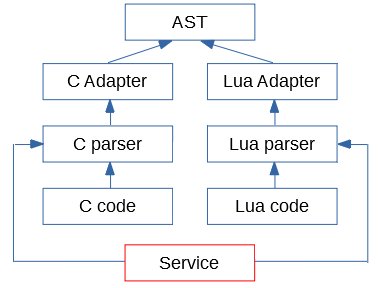
\includegraphics[scale=0.8]{images/approach_3.PNG}
        \end{figure}
        \item Prednosti: ista reprezentacija (!), nema prevođenja, proizvoljan programski jezik, mogu\'c{}e koristiti algoritme za poređenje stabala, skalabilno, samo jedan servis
    \end{itemize}
\end{frame}

\begin{frame}{Uvod i motivacija}
    \begin{itemize}
        \item Po\v{s}to nema prevođenja, mo\v{z}e se analizirati kod samo na osnovu gramatike njegovog jezika
        \item AST se dobija od stabla parsiranja izvornog koda kori\v{s}cenjem adaptera
        \item Adapteri se moraju razlikovati zbog razlika u AST
    \end{itemize}
\end{frame}

\begin{frame}{Uvod i motivacija}
    \begin{itemize}
        \item Kako pro\v{s}iriti?
        \begin{figure}[h!]
            \centering
            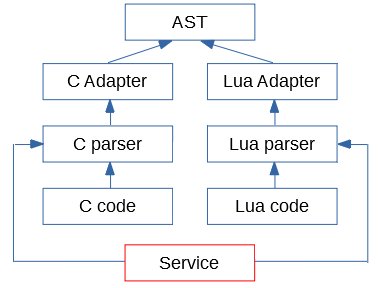
\includegraphics[scale=0.65]{images/approach_4.PNG}
        \end{figure}
    \end{itemize}
\end{frame}

\begin{frame}{AST}
    \begin{itemize}
        \item AST - Abstract Syntax Tree
        \begin{figure}[h!]
            \centering
            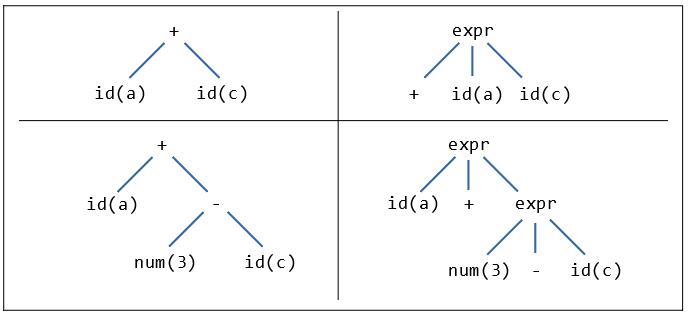
\includegraphics[scale=0.55]{images/ast.PNG}
        \end{figure}
    \end{itemize}
\end{frame}

\begin{frame}{AST}
    \begin{itemize}
        \item Go AST
        \begin{figure}[h!]
            \centering
            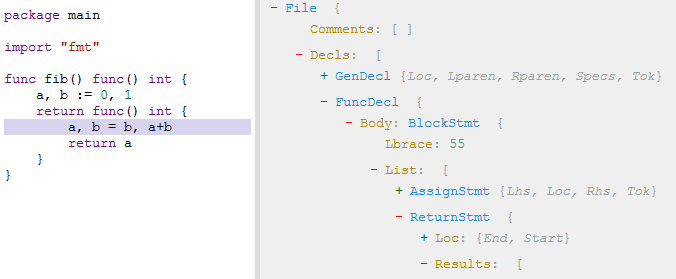
\includegraphics[scale=0.6]{images/ast_go.PNG}
        \end{figure}
    \end{itemize}
\end{frame}

\begin{frame}{AST}
    \begin{itemize}
        \item Lua AST
        \begin{figure}[h!]
            \centering
            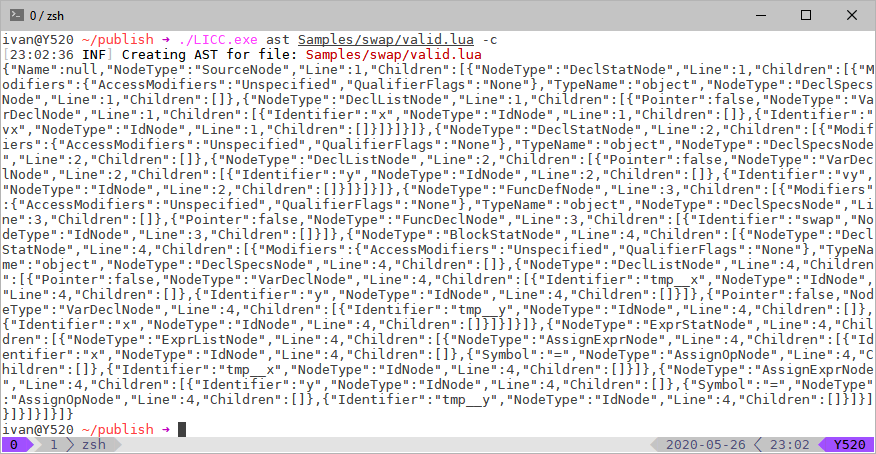
\includegraphics[scale=0.6]{images/ast_lua.PNG}
        \end{figure}
    \end{itemize}
\end{frame}

\begin{frame}{Dobijanje AST - ANTLR}
    \begin{itemize}
        \item Neophodan je parser!
        \item AST nastaje apstrahovanjem stabla parsiranja
        \item Dosta alata: Yacc, BYACC, GNU Bison, ANTLR
        \item Svi ovi alati mogu generisati parsere za proizvoljne gramatike
    \end{itemize}
\end{frame}

\begin{frame}{Dobijanje AST - ANTLR}
    \begin{itemize}
        \item \emph{ANother Tool for Language Recognition}
        \item ANTLR v4 izabran zbog:
        \begin{itemize}
            \item Mogu\'cnosti generisanja parsera u raznim jezicima (uklju\v{c}uju\'c{}i C\#)
            \item Trivijalno definisati gramatike (dosta poznatih jezika ve\'c{} podr\v{z}ano)
            \item Mogu se generisati i klase koje pru\v{z}aju interfejs za obilazak stabla parsiranja
        \end{itemize}
    \end{itemize}
\end{frame}

\begin{frame}[fragile]
\frametitle{Dobijanje AST - ANTLR}
    \begin{itemize}
        \item Prvi korak: definicija gramatike
\begin{lstlisting}[language={}]
grammar Lua;
chunk : block EOF ;
block : stat* retstat? ;
stat
    : ';'
    | varlist '=' explist
    | functioncall
    | label
    | 'break'
    | 'do' block 'end'
    | 'while' exp 'do' block 'end'
    | 'if' exp 'then' block ('elseif' exp 'then' block)* ('else' block)? 'end'
    | 'for' NAME '=' exp ',' exp (',' exp)? 'do' block 'end'
    | 'function' funcname funcbody
    ...
\end{lstlisting}
    \end{itemize}
\end{frame}

\begin{frame}[fragile]
    \frametitle{Dobijanje AST - ANTLR}
    \begin{itemize}
        \item Prvi korak: definicija gramatike
\begin{lstlisting}[language={}]
NAME
    : [a-zA-Z_][a-zA-Z_0-9]*
    ;

NORMALSTRING
    : '"' ( EscapeSequence | ~('\\'|'"') )* '"' 
    ;

WS  
    : [ \t\u000C\r\n]+ -> skip
    ;
\end{lstlisting}
    \end{itemize}
\end{frame}

\begin{frame}[fragile]
    \frametitle{Dobijanje AST - ANTLR}
    \begin{itemize}
        \item Drugi korak: generisanje parsera
\begin{lstlisting}[language={}]
$ antlr4 Lua.g4 -Dlanguage=CSharp --visitor
\end{lstlisting}
        \item Generisane \texttt{LuaLexer} i \texttt{LuaParser} klase
        \item Generisani interfejsi  \texttt{LuaListener} i \texttt{LuaVisitor}
    \end{itemize}
\end{frame}

\begin{frame}[fragile]
    \frametitle{Dobijanje AST - ANTLR}
    \begin{itemize}
        \item Tre\'c{}i korak: obi\'c{}i stablo parsiranja i kreirati AST
\begin{lstlisting}
public interface ILuaVisitor<T> : IParseTreeVisitor<T>
{
    T VisitChunk([NotNull] LuaParser.ChunkContext context);
    T VisitBlock([NotNull] LuaParser.BlockContext context);
    T VisitStat([NotNull] LuaParser.StatContext context);
    
    ...
}
\end{lstlisting}
    \end{itemize}
\end{frame}

\begin{frame}{Op\v{s}ti AST}
    \begin{itemize}
        \item \v{Z}elimo op\v{s}ti AST, koji \'c{}e podr\v{z}avati koncepte raznih imperativnih jezika
        \item Koncepti: literali, izrazi, naredbe, ...
        \item Kreirati dovoljno (ali ne previ\v{s}e) apstraktne tipove \v{c}vora za ove koncepte
        \item Specifi\v{c}nosti svesti na "ve\'c{} viđeno"
        \item Ako svođenje nema smisla, uvesti novi tip AST \v{c}vora 
        \item Izgubiti \v{s}to manje informacija!!!
    \end{itemize}
\end{frame}

\begin{frame}{Op\v{s}ti AST}
    \begin{itemize}
        \item Bazna hijerarhija
        \begin{figure}[h!]
            \centering
            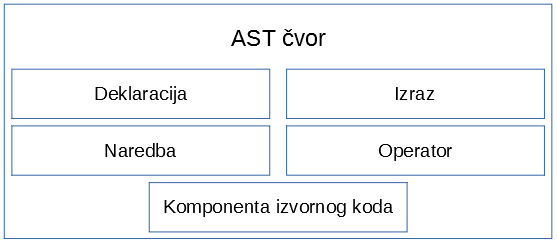
\includegraphics[scale=0.6]{images/nodes.PNG}
        \end{figure}
    \end{itemize}
\end{frame}

\begin{frame}{Op\v{s}ti AST}
    \begin{itemize}
        \item Operatori
        \begin{figure}[h!]
            \centering
            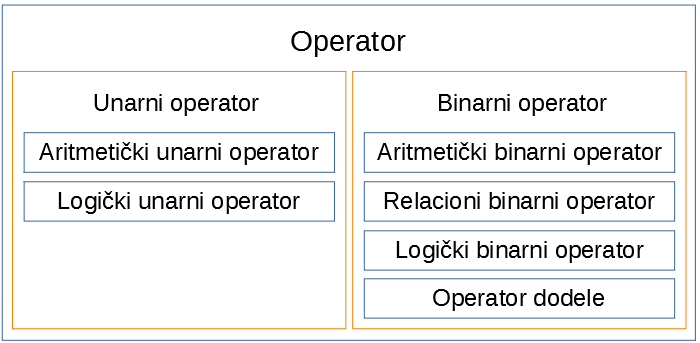
\includegraphics[scale=0.5]{images/operator_nodes.png}
        \end{figure}
    \end{itemize}
\end{frame}

\begin{frame}{Op\v{s}ti AST}
    \begin{itemize}
        \item Izrazi
        \begin{figure}[h!]
            \centering
            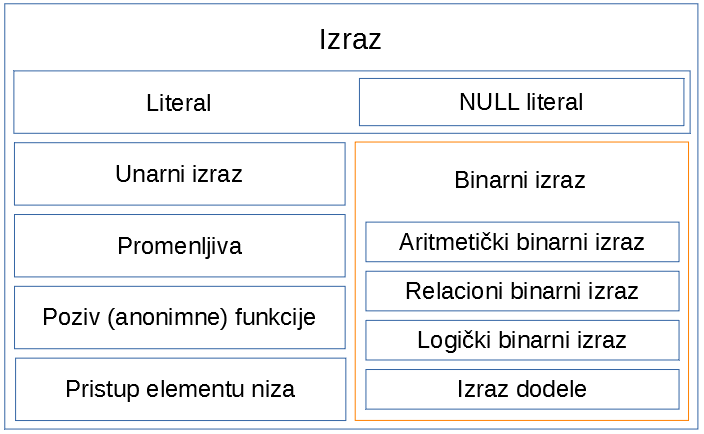
\includegraphics[scale=0.5]{images/expression_nodes.png}
        \end{figure}
    \end{itemize}
\end{frame}

\begin{frame}{Op\v{s}ti AST}
    \begin{itemize}
        \item Deklaracije
        \begin{figure}[h!]
            \centering
            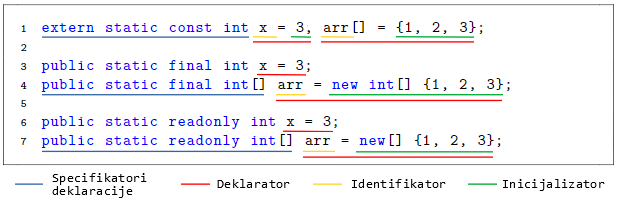
\includegraphics[scale=0.65]{images/declaration_decomposition.png}
        \end{figure}
    \end{itemize}
\end{frame}

\begin{frame}{Op\v{s}ti AST}
    \begin{itemize}
        \item Deklaracije
        \begin{figure}[h!]
            \centering
            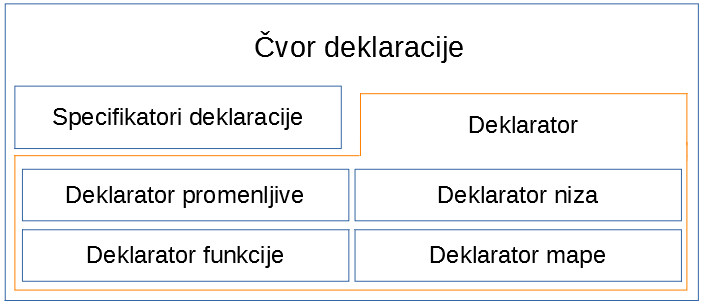
\includegraphics[scale=0.5]{images/declaration_nodes.png}
        \end{figure}
    \end{itemize}
\end{frame}

\begin{frame}{Op\v{s}ti AST}
    \begin{itemize}
        \item Naredbe
        \begin{figure}[h!]
            \centering
            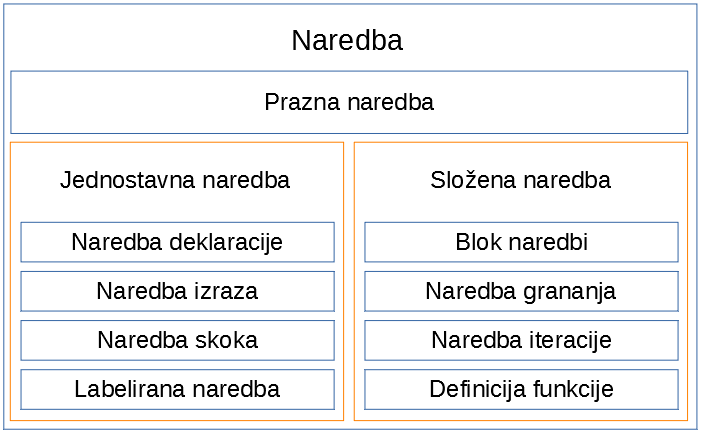
\includegraphics[scale=0.5]{images/statement_nodes.png}
        \end{figure}
    \end{itemize}
\end{frame}

\begin{frame}[fragile]
\frametitle{Op\v{s}ti AST}
    \begin{itemize}
        \item Primer - \emph{swap}
\begin{lstlisting}
int tmp = x;
x = y;
y = tmp;
\end{lstlisting}
\begin{lstlisting}
x, y = y, x
\end{lstlisting}
        \item Paziti na nove konstrukte
        \item U slu\v{c}aju skript jezika, deklarisati promenljive pre kori\v{s}\'c{}enja
    \end{itemize}
\end{frame}


\begin{frame}{Gde smo sada?}
    \begin{itemize}
        \item [x] Motivacija i uvod 
        \item [x] AST
        \item [x] Dobijanje AST - ANTLR
        \item [x] Op\v{s}ti AST
        \item [ ] Poređenje op\v{s}tih AST
        \item [ ] LICC --- Language Invariant Code Comparer
    \end{itemize}
\end{frame}

\begin{frame}{Poređenje opštih AST}
    \begin{itemize}
        \item Cilj: Napraviti pro\v{s}iriv sistem
        \item Poređenje treba da radi nad bilo koja dva \v{c}vora
        \item Ima smisla porediti samo \v{c}vorove istog tipa, ali u nekim slu\v{c}ajevima mo\v{z}da ima smisla porediti i razli\v{c}ite tipove (re\v{c}nik --- objekat)
        \item Potrebno je voditi ra\v{c}una o vrednostima promenljivih
        \item Naivno porediti \v{c}vorove stabla po jednakosti atributa i rekurzivno po jednakosti dece?
    \end{itemize}
\end{frame}

\begin{frame}[fragile]
    \frametitle{Poređenje opštih AST}
    \begin{itemize}
        \item Simboli\v{c}ko izvr\v{s}avanje 
\begin{lstlisting}
int a, b, c;

// ...

int x = 0, y = 0, z = 0;
if (a)      
    x = -2;
if (b < 5)  {
    if (!a && c)    
        y = 1;
    z = 2;
}

assert(x + y + z != 3);
\end{lstlisting}
    \end{itemize}
\end{frame}

\begin{frame}{Poređenje opštih AST}
    \begin{itemize}
        \item Simboli\v{c}ko izvr\v{s}avanje 
        \begin{figure}[h!]
            \centering
            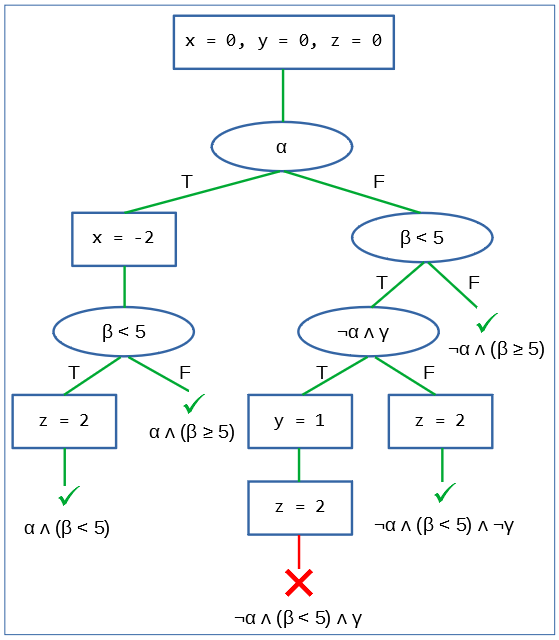
\includegraphics[scale=0.45]{images/sym_tree.png}
        \end{figure}
    \end{itemize}
\end{frame}

\begin{frame}[fragile]
    \frametitle{Poređenje opštih AST}
    \begin{itemize}
        \item Analizirati simboli\v{c}ke promenljive na kraju svakog bloka
    \end{itemize}
\begin{lstlisting}[numbers=none]
// x: 4, y: Y;
if (x > 3) {
    x = 1 + y;      
}                   // x: 1 + y | y: Y
y = 1 + x;      
                    // x: 1 + y | y: 1 + x
\end{lstlisting}
\vspace{-10pt}
\begin{lstlisting}[numbers=none]
// x: 4, y: Y;
if (x > 3) { 
    x = 1 - y;       
}                   // x: 1 - y | y: Y
y = x;
y++;
                    // x: 1 - y | y: 1 + x
\end{lstlisting}
\end{frame}

\begin{frame}{Poređenje opštih AST}
    \begin{algorithmic}[1]
        \Procedure{UporediBlokove}{$b_1$, $b_2$}
        \State $gds_1 \gets $ \emph{simboli iz svih predaka bloka $b_1$}
        \State $gds_2 \gets $ \emph{simboli iz svih predaka bloka $b_2$}
        \State $lds_1 \gets $ \emph{lokalni simboli za blok $b_1$}
        \State $lds_2 \gets $ \emph{lokalni simboli za blok $b_2$}
        \State $\text{UporediSim}(lds_1, lds_2)$
        \State $\text{IzvrsiNaredbe}(b_1, b_2, lds_1, lds_2, gds_1, gds_2)$
        \State \textbf{return} $\text{UporediSim}(lds_1, lds_2) \wedge \text{UporediSim}(gds_1, gds_2)$
        \EndProcedure
    \end{algorithmic}
\end{frame}

\begin{frame}[fragile]
    \frametitle{{Poređenje opštih AST}}
    \scriptsize
    \begin{algorithmic}[1]
    \Procedure{IzvrsiNaredbe}{$b_1$, $b_2, lds_1, lds_2, gds_1, gds_2$}
    \State $n_1 \gets $ \emph{niz naredbi bloka $b_1$} 
    \State $n_2 \gets $ \emph{niz naredbi bloka $b_2$}
    \State $i \gets j \gets 0$
    \State $ni \gets nj \gets 0$
    \State $eq \gets $ \texttt{True}
    \While{\texttt{True}}
        \State $ni \gets $ \emph{indeks prve blok-naredbe u $n_1$ počev od $ni$}
        \State $nj \gets $ \emph{indeks prve blok-naredbe u $n_2$ počev od $nj$}
        \For{$naredba \in \{n_1[x] \mid x \in [i..ni]\}$}
            \State $\text{IzvrsiNaredbu}(naredba, lds_1, gds_1)$
        \EndFor
        \State $i \gets i + ni$
        \For{$naredba \in \{n_2[x] \mid x \in [j..nj]\}$}
            \State $\text{IzvrsiNaredbu}(naredba, lds_2, gds_2)$
        \EndFor
        \State $j \gets j + nj$
        \If{$i > \text{Duzina}(n_1) \vee j > \text{Duzina}(n_2)$}
            \State \textbf{prekini petlju}
        \EndIf
        \State $nb_1 \gets $ \emph{izvuci blok iz naredbe $n_1[i]$}
        \State $nb_2 \gets $ \emph{izvuci blok iz naredbe $n_2[j]$}
        \State $eq \gets eq \wedge \text{UporediBlokove}(nb_1, nb_2)$
        \State $i \gets i + 1$
        \State $j \gets j + 1$
    \EndWhile
    \State \textbf{return} $eq$
    \EndProcedure
    \end{algorithmic}
\end{frame}

\begin{frame}{Pitanja}
    \centering
    ???
\end{frame}

\end{document}
